% Why prediction is important?
\label{sec:prediction}
This section further motivates predictive false sharing and explains how to support it in the runtime system.  

\subsection{Overview}
%\begin{figure*}[!htb]
\label{sec:predictoverview}

\begin{figure}[!t]
\begin{center}
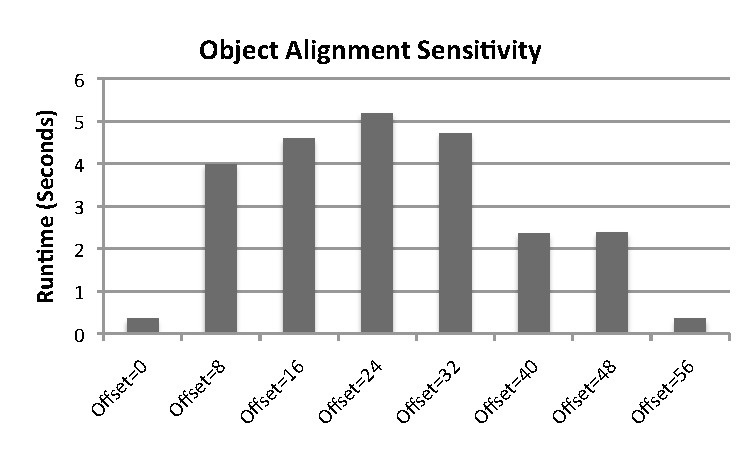
\includegraphics[width=6in]{predator/figure/perfsensitive}
\end{center}
\caption{
Performance of the linear\_regression benchmark from the Phoenix benchmark suite.
Performance is highly sensitive to the offset of the starting address of the (potentially) falsely-shared object 
and the start of cache line. 
\label{fig:perfsensitive}}
\end{figure}

The appearance of false sharing depends on 
the alignment between objects and corresponding cache lines.
A real example, linear\_regression, is shown in Figure~\ref{fig:perfsensitive}.
For this benchmark, when the offset of the starting address between the potentially falsely-shared object and corresponding cache lines is $0$ or $56$ bytes, 
there is no false sharing. 
When the offset is $24$ bytes, we see the most severe performance effect caused by false sharing. 
The performance difference between these two scenarios can be as large as $15\times$. 

Existing detection tools can only report observed false sharing. For this case, they may miss a very severe false sharing problem that could occur in the wild if the offset of the starting address was $0$ bytes or $56$ bytes in their test environment.
\Predator{} overcomes this shortcoming by accurately predicting potential false sharing.

\begin{figure*}
\begin{center} 
\subfigure[No false sharing]{%
   \label{fig:nofs}
   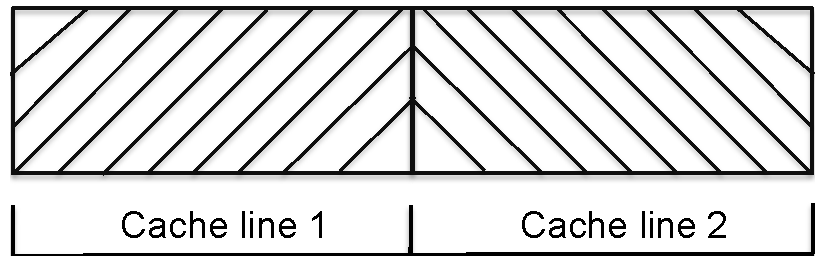
\includegraphics[width=0.24\textwidth]{predator/figure/Potential1}
}%
\hspace{10pt}
\subfigure[False sharing with larger cache size]{%
   \label{fig:fslarger}
   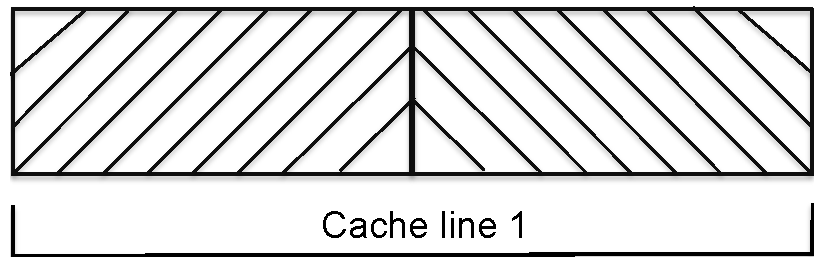
\includegraphics[width=0.24\textwidth]{predator/figure/Potential2}
}%
\hspace{10pt}
\subfigure[False sharing with different memory layout]{%
   \label{fig:fsnoalignment}
   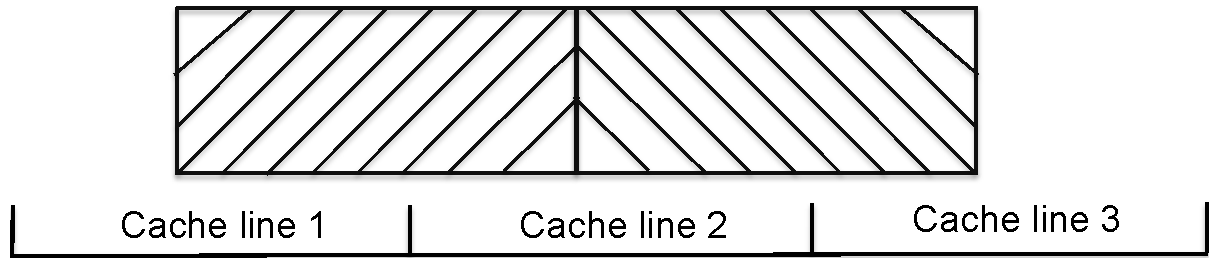
\includegraphics[width=0.36\textwidth]{predator/figure/Potential3}
}%
\end{center}
%\includegraphics{fig/potential.pdf}
\caption{False sharing under different environments.}
\label{fig:potentialfalsesharing}
\end{figure*}

\Predator{} predicts {\it potential false sharing}, the type of false sharing that does not manifest in the current execution but may appear and greatly affect programs' performance in a slightly different environment.

Figure~\ref{fig:potentialfalsesharing} shows a simplified example why occurrences of false sharing 
can change in different situations.
In this figure, two rectangles with different patterns
represents two portions of the same object, updated by different threads. 
In Figure~\ref{fig:nofs}), there is no false sharing when thread T1 only updates 
``cache line 1'' and T2 only updates ``cache line 2''.
However, false sharing appears in one of the following cases, even with the same
access pattern. 

\begin{itemize}
\item
Doubling cache line size (Figure~\ref{fig:fslarger}). When the size of a
cache line doubles,
both T1 and T2 access the same cache line and false sharing occurs in this case.

\item
Different starting address of an object(Figure~\ref{fig:fsnoalignment}). 
When the starting address of this object is not aligned with the starting address of 
the first cache line, 
then T1 and T2 can update the second cache line simultaneously, 
causing false sharing. 
%When some dynamic property changes the starting address of this object so that it 
%is not aligned with the starting address of the first cache line, 
\end{itemize} 

\Predator{} predicts whether programs can have potential false sharing  
in either of these two cases, where they can be caused by different dynamic properties 
discussed in Section~\ref{sec:intro}.
All dynamic properties, except the change of cache line size,
can lead to different starting address of an object. 
Thus, predicting false sharing in these two cases actually 
explores many possibilities caused by all dynamic properties.

\subsection{Basic Prediction Workflow}
\label{sec:predictionmechanism} 

%Similar to the detection part, 
\Predator{} focuses exclusively on potential false sharing that can 
cause performance problems.
The implementation is based on
two key observations. First, only accesses to 
adjacent cache lines can form potential false sharing, 
i.e., introducing cache invalidations when cache line size
or an object's starting address changes.
Second, only when false sharing introduces a large number of cache invalidations
can it degrade performance.

Based on these two observations, \Predator{} develops 
the following workflow to capture potential false sharing.
Those detection optimizations listed in Section~\ref{optimization} can also be applied
to prediction part. We do not repeat these optimizations in this section.

\begin{enumerate}
\item
Track the number of writes on different cache lines. 

\item
When the number of writes to a cache line $L$ reaches {\it Tracking-Threshold},
track the detailed read and write accesses for every word on both cache line $L$ 
and its adjacent cache lines. 

\item
When the number of writes to a cache line $L$ reaches a second threshold (called as
{\it Predicting-Threshold}), 
identify whether there exists false sharing in $L$ and its adjacent 
cache lines by analyzing word accesses information collected in Step 2. 
Section ~\ref{sec:evaluatingfs} describes the evaluation method.

\item
If a potential false sharing is found, continue to track cache line invalidations to confirm it. Section~\ref{sec:tracking} discusses the details.
Otherwise, go back to Step 2 to track more detailed accesses.
 
\end{enumerate}

\subsection{Searching for Potential False Sharing}
\label{sec:evaluatingfs}
To describe potential false sharing in two different cases, we first 
introduce the concept of a virtual cache line.  A virtual cache line
is a contiguous memory range that spans one or more physical cache 
lines.  In the case of double cache line size, a virtual line is
composed of two original contiguous cache lines and the first cache
line has an even index number.  Thus, only cache lines $2*i$ and
$2*i+1$ can form a virtual line.  In the case of different starting
addresses, a virtual line can have the same size as physical lines,
but can be positioned arbitrarily: unlike actual cache lines, the
starting address of a virtual cache line does not need to be multiple
of the cache line size.  For instance, a 64-byte long virtual line can
consist of the range $[0,64)$ bytes or $[8,72)$ bytes.

To search for potential false sharing problems, 
\Predator{} searches for a hot access pair on $L$ and its adjacent cache lines 
by analyzing the detailed word access information collected in Step 2. 
A hot access in a cache line refers to the word whose number of read or write accesses 
is larger than the average number of accesses to each word of cache line $L$.
For every hot access $X$ in cache line $L$, \Predator{} searches another
hot access $Y$ in $L$'s previous cache line or next cache line satisfying
the following conditions: 

\begin{itemize}
\item
$X$ and $Y$ reside on the same virtual line. 

\item
One of $X$ and $Y$ is a write access.

\item 
$X$ and $Y$ are issued by different threads.

\end{itemize}

% why it finds a pair of $X$ and $Y$ == a potential false sharing 
Whenever it finds such a pair $X$ and $Y$, 
\Predator{} identifies potential performance-degrading false sharing whenever
 the number of cache invalidations caused by $X$ and $Y$, at a possible virtual line, 
is larger than the average number of accesses on each word of $L$. 
This approach is based on a similar observation as in detection:
\emph{if a thread writes a virtual line after other threads 
have accessed the same virtual line, this write operation most likely causes at least one cache 
invalidation}. 
Before tracking detailed memory accesses on a virtual line, it is impossible to know exactly how many cache invalidations happen on a virtual line. Thus, \Predator{} conservatively assumes that accesses from different threads occurs interleavedly.
This approach ensures that \Predator{} does not miss any potential false sharing as well as 
not reporting false positives. 

%According to above observation and assumption, 
%a pair of hot accesses, $X$ and $Y$, if accesses are issued in an interleaving 
%way, can generate the number of cache invalidations equaling to 
%the smaller number of accesses of $X$ and $Y$.
%Thus a false sharing problem is to be identified by \Predator{}.
  
After identifying possible false sharing, \Predator{} goes to Step 4 to 
verify whether this is an actual false sharing problem.

\subsection{Verifying Potential False Sharing}
\label{sec:tracking}

\Predator{} verifies potential false sharing by tracking 
cache invalidations on a problematic virtual line.
%covering a pair of hot accesses found
%in Step 3.

For potential false sharing caused by double cache line size, as described in
Section~\ref{sec:evaluatingfs}, a virtual line is always composed of 
cache line with index $2*i$ and $2*i+1$. 
\Predator{} tracks cache invalidations
on the virtual line on which false sharing has been discovered.

However, for the case of a change in starting address,
two hot accesses with distance less than cache line size 
can form multiple virtual lines. 
There is thus an additional step to determine which virtual line to be tracked.
Although the virtual line to be chosen here is never a real cache line of actual hardware
because of unaligned addresses,
we utilize this virtual line to simulate the effect of changing the 
starting addresses of objects.


\begin{figure}
\begin{center} 
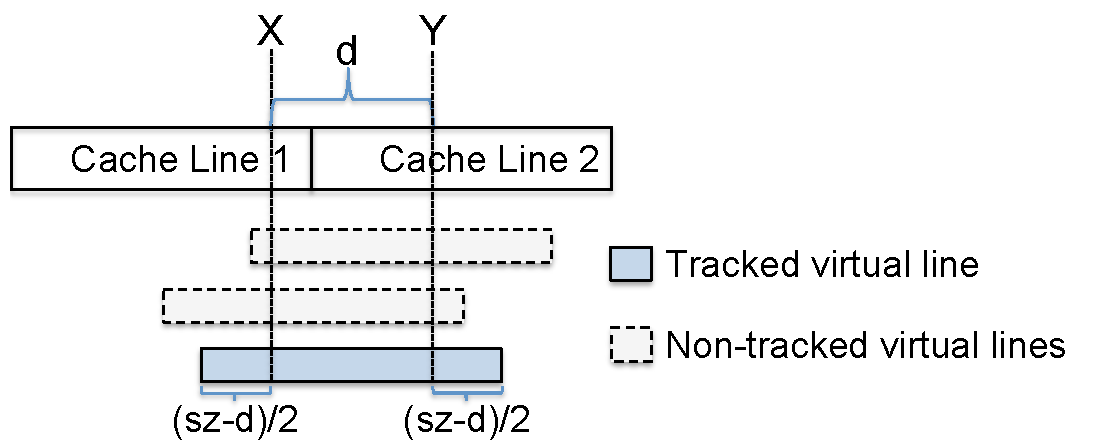
\includegraphics[width=6in]{predator/figure/trackpotential}
\end{center}
\caption{Determining a virtual line with size $sz$ according to hot accesses.}
\label{fig:trackpotential}
\end{figure}

Given two words with the hot accesses shown in Figure~\ref{fig:trackpotential}, 
\Predator{} leaves the same space before $X$ and after $Y$ in determining a virtual line. 
That is, the virtual line starting 
at location $X-((sz-d)/2)$ and ending at $Y+((sz-d)/2)$ is tracked. 
This choice allows tracking of more possible cache invalidations caused by
adjacent accesses of $X$ and $Y$. 
Since adjusting the starting address of a virtual line has the same effect of
adjusting the starting address of an object in detecting false sharing,
all cache lines related to the same object must be adjusted at the same time.
\Predator{} then tracks cache invalidations based on these adjusted virtual lines.

